%%% Setup %%%
\documentclass{article}
\usepackage{program}
\usepackage{acm-style10} % ACM proceedings formatting
\usepackage{times}       % Use Adobe Times font set
\usepackage{epsfig,twocolumn}
\usepackage{url}
\usepackage[english]{babel} % mdw: Required to get good hyphenation on RH6.0
                            % (fixed in RH6.1)
\usepackage{graphicx} 
\graphicspath{ {figures/} }
\usepackage{color}


\usepackage{hyperref}


% DO NOT EDIT THE BELOW BLOCK OF CODE
\def\dsp{\def\baselinestretch{1.10}}
\dsp
\newcommand{\XXXnote}[1]{{\bf\color{red} XXX: #1}}
\setlength{\textheight}{9.25in}
\setlength{\columnsep}{0.33in}
\setlength{\textwidth}{7.4in}
\setlength{\footskip}{0.0in}
\setlength{\topmargin}{-0.25in}
\setlength{\headheight}{0.0in}
\setlength{\headsep}{0.0in}
\setlength{\oddsidemargin}{-.45in}
\setlength{\parindent}{1pc}
\pagestyle{empty}

\usepackage{listings}
\lstset{language=C}
\lstset{
	language=C,
    frame=L,
    captionpos=b,
    tabsize=2,
    basicstyle=\ttfamily\scriptsize,
    breaklines=true
}

\title{A Comparison of Concurrency in Rust and C}
\author{
    Josh Pfosi\\joshua.pfosi@tufts.edu
    \and
    Riley Wood\\riley.wood@tufts.edu
    \and
    Henry Zhou\\henry.zhou@tufts.edu
}
\date{}


\begin{document}
\maketitle

\begin{abstract}
\begin{small}
As computer architects are unable to scale clock frequency due to a power wall, parallel architectures have begun to proliferate. With this shift, programmers will need to write increasingly concurrent applications to maintain performance gains. Parallel programming is difficult for programmers and so Rust, a systems programming language, has been developed to statically guarantee memory- and thread-safety and catch common concurrency errors. This work draws comparisons between the performance of concurrency features and idioms in Rust, and the low level and distinctly unsafe implementation of Pthreads in C. We find that while Rust catches common concurrency errors and does not demonstrate additional threading overhead, it generally executes slower than C and exhibits unintuitive locking behavior.
\end{small}
\end{abstract}

%%% The Meat %%%

\section{Introduction}\label{sec::introduction}

As the "power wall" has stalled advances in clock frequency, the industry has begun to favor parallel architectures to improve performance~\cite{sutter2005free}. This shift has significant ramifications for
programmers. A program’s performance scales trivially with clock frequency, whereas parallel programs
often require significant design effort on the part of the programmer to scale well. But if software performance is to improve in step with hardware, concurrent software must become the norm. It is difficult for most programmers to decompose an algorithm into parallel workloads and to anticipate all of the interactions that
can occur. This proliferates new kinds of errors that are much harder to anticipate, find, and prevent including deadlock, livelock, and data races. Much work has been done analyzing the nature of, locating, and reproducing these common programmer errors~\cite{kendo,grace,ctrigger,heisenbug,learning}. Many common concurrency challenges, however, have not conclusively been solved for programmers.

It is important that programmers start writing parallel programs in order to scale software performance with hardware. To this end, programmers should feel confident in their ability to write safe, parallel code. The question becomes: Which tools currently available are best suited for the task? One technique that has had moderate success is the development of thread-safe programming languages to help programmers better express their intentions and avoid common mistakes~\cite{learning}.

The goal of this paper is to analyze one such language, Rust, a new systems programming language that aims to help programmers write concurrent code with zero-cost abstractions~\cite{rust-lang}. Designed to be a modern, open-source systems programming language, Rust leverages a powerful type system to make static guarantees about program safety. Rust allows for manual memory management similar to C, but it employs several special rules at compile time regarding variable bindings and memory allocation. One rule that Rust enforces is the concept of \textit{ownership} to ensure memory safety. When a variable binding is assigned, such as \texttt{let x = y}, the ownership of the data referenced by \texttt{y} is transferred to \texttt{x}. Any subsequent usages of \texttt{y} are invalid. In this way, Rust enforces a one-to-one binding between symbols and data. Ownership is also transferred when passing data to functions. Data can be borrowed, meaning it is not deallocated when its binding goes out of scope, but the programmer must make this explicit. Data can be borrowed as mutable or immutable, also specified explicitly, and the compiler makes sure that permissions to borrowed data are not violated by the borrower. Furthermore, the Rust compiler enforces the notion of \textit{lifetimes}, which ensures when a binding falls out of scope, the reference is deleted from the stack and its data is de-allocated from the heap. This means that dangling pointers are no longer a danger to programmers. With ownership, borrowing, and lifetimes, Rust forces the programmer to make promises about how they will share and mutate data which are checked at compile time. These constraints have serious implications for concurrent programming, as we discuss in Section~\ref{sec::rust_concurrency}. We are interested in assessing whether or not they impact the performance of concurrency in Rust.

For comparison, we have selected the C programming language and the Pthreads API. We chose C as it is a natural competitor to Rust, and its (lack of) safety features and threading paradigms are well known. Further, many parallel programming errors specifically caught by the Rust type system are made often in C.
The remainder of this paper explores the tradeoffs made by the Rust programming language in terms of usability and performance with respect to C implementations using Pthreads. Section~\ref{sec::relatedwork} summarizes related projects which address concurrent programming challenge, Section~\ref{sec::methodology} discusses our experimental methodology, Section~\ref{sec::results} describes our findings, and Section~\ref{sec::conclusion} concludes.

\section{Concurrency in C}
The C parallel programming paradigm follows directly from its design philosophy: low level and unsafe, in the sense that the programmer is trusted to write safe code. Because C does not check pointer operations, C programs can cause notorious problems such as use-after-free bugs. Common pitfalls such as data races and deadlock can easily go unnoticed and must be avoided by adhering to “good practice” conventions. The hazards posed by concurrent programming in C are easy to run into and potentially limit the scalability of concurrent software written in C. This manifests strikingly in most modern browsers which are struggling to benefit from multiprocessor devices as their core rendering engines are written as single-threaded C++ monoliths~\cite{servo}.
\section{Concurrency in Rust}\label{sec::rust_concurrency}
Rust's guarantees memory safety, efficient C bindings, and data-race free threading at compile time. Multithreading in Rust is available through its standard library. Threads are spawned using a thin wrapper around Pthreads. Syntactically, threads in Rust execute a closure. A handle is returned when a thread is spawned, similar to a \texttt{pthread\_t} in C.

In order to help programmers write and reason about concurrent code, Rust offers a static type system with the concept of traits. Traits tell the Rust compiler about the functionality that a type must provide, and there are two key traits that matter for concurrent programming. The first is \texttt{Send}. \texttt{Send}-compliant types can have their ownership safely transferred between threads; types that do not implement \texttt{Send} are not guaranteed to be thread-safe and will not be allowed to be sent from one thread to another. The second property is \texttt{Sync}, which guarantees that concurrent accesses from multiple threads to the same data structure are safe. In other words, the threads' access to the \texttt{Sync} data is mutually exclusive. As an example, Rust implements mutexes using the \texttt{Sync} property.

Often, multithreading in C involves passing pointers to the same data to different threads, creating a potential data race depending on the threads' access pattern. Rust's type system prevents threads from directly sharing references to the same memory. Instead, Rust mandates that such sharing be managed by the \texttt{Arc<T>} type, an atomic reference count type. \texttt{Arc}s keep track of how many threads have access to the data they contain so that they know when the data falls out of scope and can be deallocated. For \texttt{Arc<T>} to be passed to threads, it and its contents must implement \texttt{Send} and \texttt{Sync}. For immutable values, both characteristics are guaranteed. However, the \texttt{Sync} property is not inherently implemented by mutable values because a data race is possible. Consequently, mutable values must first be stored within a \texttt{Mutex<T>} , which only allows one thread to hold the lock to access its reference.

The \texttt{Mutex<T>} type is similar to \texttt{pthread\_mutex\_t}, but it differs in that it wraps the data which it protects unlike the \texttt{pthread\_mutex\_t} which wraps sections of code. This echos Rust's design philosophy to ``lock data, not code''~\cite{rust-lang}. The idea is that linking the mutex to the data it protects limits misuse and deadlock. From the programmer's perspective, there are similarities between the usage of \texttt{std::thread}s in Rust and Pthreads in C, but Rust's enforcement of ownership with mutable state, and type system ensure that threaded processes will be memory safe and free of race conditions.
\section{Work Related to Rust}\label{sec::relatedwork}
Other languages take a slightly different approach than Rust to making concurrent programming easier. Rust's own developers admit that Rust is "not particularly original", borrowing many of its design elements from a variety of languages~\cite{rust-influences}. Library based solutions such as OpenMP~\cite{openmp} and CILK/CILK++~\cite{cilk} facilitate writing scalable multithreaded solutions via compiler directives, language extensions and sophisticated runtime systems which schedule threads, balance load, and manage inter-thread communication. Ivory is another programming language with similar design goals to Rust~\cite{ivory}. Designed for high-assurance applications, Ivory is embedded within a variant of Haskell and compiles directly to C. To guarantee memory safety, however, Ivory limits functionality in critical ways, such as:
\begin{itemize}
\item Heap allocation is forbidden
\item All loop iterations must be statically bounded by a constant
\item Expressions must have no side-effects
\end{itemize}
These limitations severely limit expressive power and common programming idioms, but further underscore the importance of memory safety in systems programming. Ivory's design as well as the OpenMP and CILK projects show that there is interest in addressing the same problems that Rust tackles.
\section{Methodology}\label{sec::methodology}

To achieve our goal of comparing concurrency frameworks in Rust and in C, we selected concurrency frameworks for each language. For C, we chose the raw Pthreads library as this was sufficiently low level, simple to program with and reason about, and ubiquitous among programmers. Also, it does not require an additional runtime system like other solutions such as OpenMP or CILK. For Rust, we chose the standard library solution, \texttt{std::thread}, except one benchmark for which we used the \textit{crossbeam} threading library.
%The motivation for this choice was discussed in section~\ref{sec::rust_concurrency}.

As of Rust 1.0-alpha~\cite{rust-release}, the language removed support for green threading, and instead uses “native OS threads”~\cite{rust-doc}. Rust wraps Pthreads, an inherently unsafe library, with its \texttt{std::thread} library, leveraging its safety features. Consequently, our measurements characterize the efficacy of Rust's use of Pthreads compared to a hand-crafted C implementation.

This research attempts to answer: \textit{Does Rust's concurrency framework, with its emphasis on safety, come with drawbacks that outweigh its usefulness?} To explore this question we sought benchmarks which captured common parallel programming techniques. We chose three: blackscholes (from the PARSEC benchmark suite \cite{parsec}), matrix multiplication, and vector dot product. As programmers most familiar with C/C++, we experienced the semantic differences between Rust and C and gained insight into how Rust's strict compiler may hinder a programmer who takes a typical C approach to implementing a concurrent algorithm. Therefore, a second question we seek to answer is: \textit{Does Rust's insistence on safety unnecessarily hinder a skilled concurrent programmer?}

To measure our benchmarks, we used the Sniper Multi-Core Simulator~\cite{sniper}. We simulated an 8 core machine based on the Nehalem architecture. We ran the benchmarks in serial, avoiding calls to the concurrency frameworks, and then with two, four and eight threads. Our benchmarks invoke the relevant number of threads from the main thread of execution, which then waits for the spawned threads to complete. We took steps to make sure the data access patterns of each benchmark in C and Rust were kept the same. To hone in on the performance of the kernel itself, we took advantage of Sniper's ``region of interest'' feature, which enables us to hone in on the parallelized portions of the benchmarks.

\subsection{Our Benchmarks}
\subsubsection{Matrix Multiplication}
We measure the performance of matrix multiplication to examine how each language's concurrency framework handles shared data structures between threads. The benchmark multiplies a matrix $M$ by itself, where $M$ is a matrix of 128 x 128 unsigned integers with values $0, 1, \dots, 127$. This benchmark's Rust implementation differs from our other Rust benchmarks in that we use the \texttt{crossbeam} threading library to parallelize the kernel, rather than \texttt{std::thread}s. This is because we encountered difficulties sharing the output matrix between threads using \texttt{std::thread}s. This shed light on the ways Rust's constraints can restrict the programmer in unexpected ways. We will discuss the development of this benchmark and the switch from \texttt{std::thread}s to \texttt{crossbeam} in Section~\ref{sec::results}. Matrix multiply is a good benchmark to use as it tests both memory access behavior as well as a series of arithmetic operations.

\begin{lstlisting}[caption={Matrix Multiply C kernel}]
void* multiply(void* slice)
{
  int s = (int)slice;   // retrive the slice info
  int from = (s * SIZE)/num_thrd; // note that this 'slicing' works fine
  int to = ((s+1) * SIZE)/num_thrd; // even if SIZE is not divisible by num_thrd
  int i,j,k; 
  for (i = from; i < to; i++)
  {  
    for (j = 0; j < SIZE; j++)
    {
      C[i][j] = 0;
      for ( k = 0; k < SIZE; k++)
      {
      	C[i][j] += A[i][k]*B[k][j];
      }
    }
  }
  return 0;
}
\end{lstlisting}

\begin{lstlisting}[caption={Matrix Multiply Rust kernel}]
for i in from..to {
    for j in 0..TOTAL_SIZE {
        for k in 0..TOTAL_SIZE {
            chunk[count] += a[i][k] * b[k][j];
        }
        count += 1;
    }
}

\end{lstlisting}
\subsubsection{Blackscholes}
Blackscholes is a popular benchmark that is part of the PARSEC parallel programming benchmark suite \cite{parsec}. It is a financial application that simulates options pricing using the Black-Scholes partial differential equation. We chose this benchmark because it is widely studied and presents a practical application of concurrent programming.
To port blackscholes to Rust, we took advantage of Rust's ability to link with C libraries~\cite{rustlinking}. We compiled the blackscholes kernel from PARSEC as a shared library, and linked to it from our Rust code with the \textit{\#link} attribute. At that point, we were able to parallelize calls to the blackscholes kernel using Rust \texttt{std::thread}s.
For our C tests, we compiled serial and parallel versions of the blackscholes benchmark using the \texttt{parsecmgmt} tool that ships with PARSEC.
The code for the blackscholes kernel can be found in the PARSEC benchmark suite source code.

\subsubsection{Dot Product}
Our dot product benchmark computes the dot product of two vectors of $2^{20}$ double-precision values. We measured dot product to explore how Rust's \texttt{Arc} and \texttt{Mutex<T>} type impacts embarrassingly parallel tasks compared to a \texttt{pthread\_mutex\_t} in C. We implemented dot product in two ways. In one implementation, threads compute local sums that are summed together after the threads complete. In the other, threads concurrently add to a global sum, in which case a mutex is required. This allows us to investigate the performance of locks in Rust as compared to C. 


\begin{lstlisting}[caption={Dot Product C Kernel}]
void *dotprod(void *arg)
{
    int i, start, end, len ;
    long tid;
    double partialsum, *x, *y;
    tid = (long)arg;

    len = dotstr.veclen;
    start = tid * len;
    end   = start + len;
    x = dotstr.a;
    y = dotstr.b;

    partialsum = 0;
    for (i = start; i < end ; i++)
    {
        partialsum += (x[i] * y[i]);
    }

    dotstr.sum[tid] = partialsum;

#if NTHREADS != 1
    pthread_exit((void*) 0);
#else
    return NULL;
}
\end{lstlisting}

\begin{lstlisting}[caption={Dot Product Rust Kernel}]
fn dot_prod(x: & Vec<f64>, y: & Vec<f64>, start: usize, end: usize) -> f64 {
     let mut dotprod: f64 = 0.0;
     for i in start..end {
         if i < x.len() {
             dotprod = dotprod + (x[i] * y[i]);
         }
    }
     dotprod
 }
\end{lstlisting}
\section{Results \& Analysis}\label{sec::results}

\subsection{Comparing Performance}
We seek to evaluate the overhead of each language's concurrency framework. Therefore, we present the normalized speedup as a function of the number of threads for each benchmark implementation from 1 to 8 threads in Figure~\ref{fig:speedup}. 
\begin{figure}
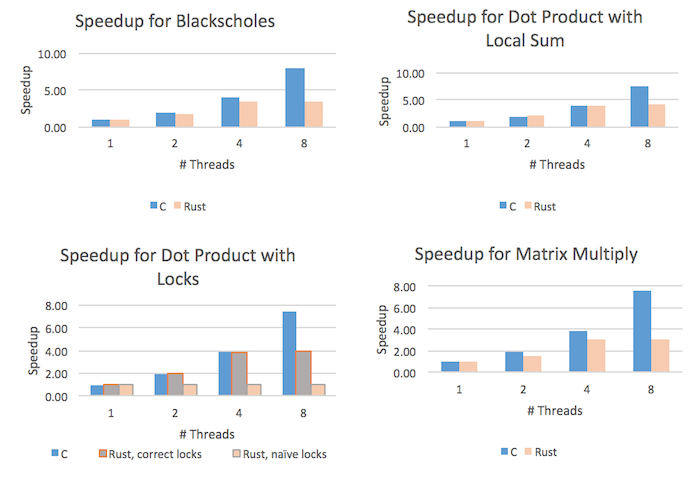
\includegraphics[scale=0.4]{speedup_benchmarks}
\caption{Speedup in each language}
\label{fig:speedup}
\end{figure}

\begin{figure}
\centering
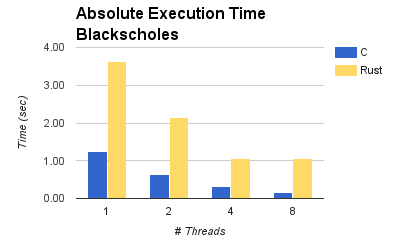
\includegraphics[width=0.45\textwidth]{blackscholes_abs.png}
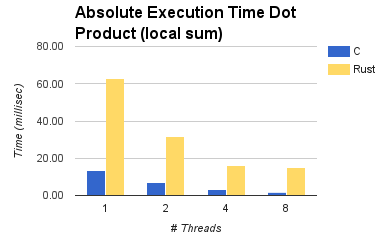
\includegraphics[width=0.45\textwidth]{dot_product_local_abs.png}
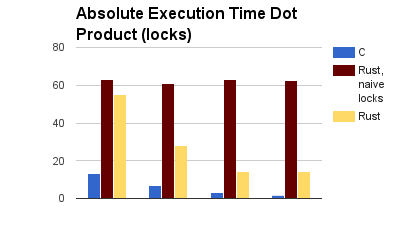
\includegraphics[width=0.45\textwidth]{dot_product_locks_abs.png}
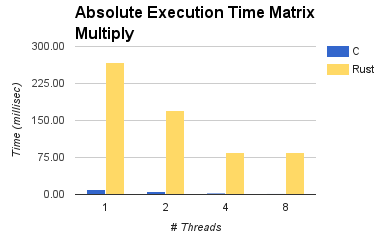
\includegraphics[width=0.45\textwidth]{mm_abs.png}
\caption{Execution of blackscholes for 1 to 8 threads on a reference Linux 8 core machine.}
\label{fig:absolute_time}
\end{figure}

The speedup ideally scales with the number of threads. One can see that C very nearly achieves this in every benchmark. Rust keeps up best in both implementations of dot product, fairly well in blackscholes, and less so in matrix multiply.

Figure~\ref{fig:absolute_time} displays our absolute execution times recorded for the four benchmarks. Generally speaking, C still dominates Rust by a relatively wide margin in terms of execution time. Consequently, there is definitely a performance cost associated with using Rust instead of C. In spite of this, Rust's execution time halves every time the number of threads is doubled for 1 through 4 threads, which corresponds to the doubling of speedup as observed in Figure 1.

A striking result from our Sniper simulations is that at 8 threads, on an 8 core machine, Rust lags behind C egregiously. Figure~\ref{fig:instr_load} shows that this is due to a workload imbalance that only afflicts our Rust benchmarks. One can see that for each Rust benchmark, core 0 is largely idle while another core takes on twice the work as the others and thus slows down the entire program. Hence our slowdown at eight threads in Sniper.

We investigated this discrepancy further by running the Rust blackscholes benchmark on an 8-core physical machine to see if this problem was merely an artifact of the Sniper simulator. Figure~\ref{fig:baremetal} shows that on a physical machine, normalized speedup continues to improve at eight threads, contradicting our simulator results from Figure~\ref{fig:speedup}. Admittedly, because we were unable to isolate the parallel region of interest on our physical machine, we see diminishing returns in speedup as the number of threads increases, as described by Amdahl's Law. Still, we have conclusively determined that the Sniper scheduler is giving erroneous results for Rust at eight threads due to some issue with its scheduler. It is interesting that this problem in Sniper occurs only with our Rust programs, not our C programs. Nevertheless, because of this simulator error, we feel it is best to ignore the data point for speedup at eight threads in Figure~\ref{fig:speedup}.
\begin{figure}
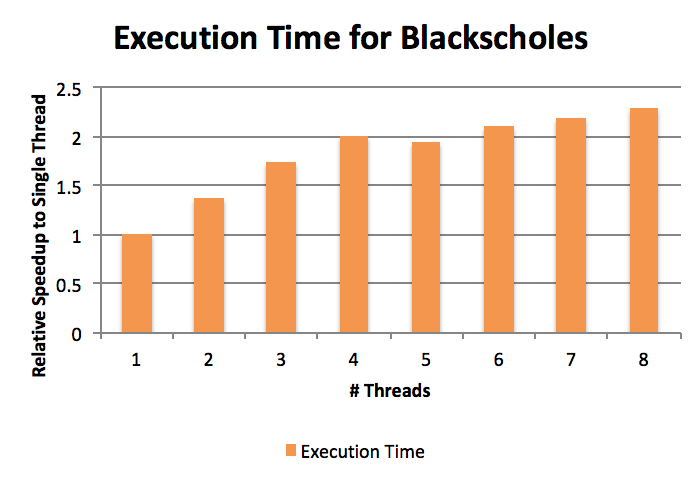
\includegraphics[scale=0.7]{relative_speedup}
\caption{Execution of blackscholes for 1 to 8 threads on a reference Linux 8 core machine.}
\label{fig:baremetal}
\end{figure}

\begin{figure}
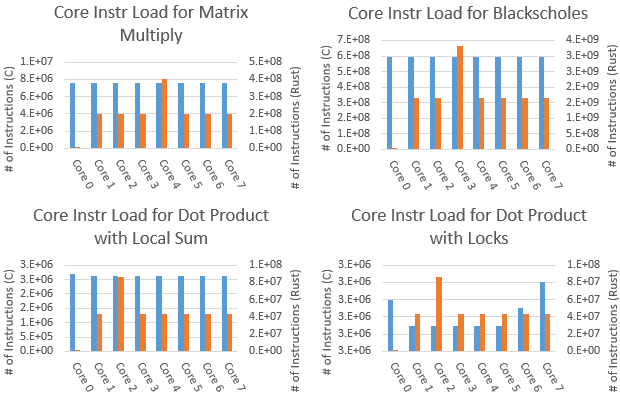
\includegraphics[scale=0.4]{instr_benchmarks}\\
\caption{Instruction load per core at eight threads running in Sniper}
\label{fig:instr_load}
\end{figure}

Additionally, a compelling ``gotcha'' we uncovered was the unexpected slowdown of the Rust dot product benchmark when unwrapping and modifying locked data in one line. To ensure memory safety, the Rust compiler emits synchronization code (as well as other memory management code e.g. destructors) around accesses to objects of type \texttt{Mutex<T>}. In our dot product benchmark's original implementation, the result of the parallel dot product computation was used as an rvalue for an addition operation on a synchronized variable (see Listing~\ref{list:rvalue}).

\begin{lstlisting}[caption={Rvalue used in serialized add},label=list:rvalue]
*dotprod_shared.lock().unwrap() +=
			dot_prod(&x_shared, &y_shared, start, end);
\end{lstlisting}

This unexpectedly serialized the computation of the rvalue as well such that no benefit came from parallelization, as shown by the flat line labeled "naive locks" in Figure~\ref{fig:speedup}. Ideally, the compiler would compute the rvalue before attempting to unlock the lvalue so that the program would not be serialized. This problem was solved by expressing the above in two lines, as shown in Listing~\ref{list:2line}.
\begin{lstlisting}[caption={Rvalue used in serialized add},label=list:2line]
let thrdsum = dot_prod(&x_shared, &y_shared, start, end);
*dotprod_shared.lock().unwrap() += thrdsum;
\end{lstlisting}

\subsection{Comparing Ease of Implementation}
Although Rust's ownership system ensures memory safety and synchronization of data, there exists a learning curve that must be overcome. As newcomers to the Rust language, we had difficulties complying with the ownership system at first. However, over time we began to appreciate Rust as it forces the programmer to consider the safety of their code. In the same vein, Rust forces the programmer to think about parallel memory safety. However, there are still some annoyances about Rust that can, at times, make implementing a simple algorithm difficult.

For example, we found Rust's insistence on avoiding any possibility of a data race to be cumbersome at times. In the matrix multiplication benchmark, each thread is given exclusive access to a section of a shared data structure. Rust prevents the data structure from being shared across multiple threads for fear of a data race, even though accesses are mutually exclusive in our algorithm. In C, this is of course not a problem, but we found Rust's strictness to be a hindrance.

We looked to other threading libraries as a way of circumventing this issue. We settled upon \texttt{crossbeam}'s scoped threads as a way of statically specifying the portion of the output matrix that each thread could mutate. This way, we could implement our algorithm as we did in C, and the Rust compiler could be guaranteed that accesses to regions of the data structure were mutually exclusive. Initial debugging of this issue proved to be painful because of nebulous compiler errors and our lack of Rust expertise, but integration of the library to implement the fix was easy thanks to Rust's \texttt{cargo} package manager.

Overall, we found that in this instance, writing safe Rust code was more of a hassle than beneficial, since we knew in advance that our chosen algorithm was thread-safe. In this case, it may have been appropriate to use Rust's \texttt{unsafe} tags to surround concurrent accesses to the shared output matrix, but in retrospect we feel it was worthwhile to see the lengths one would need to go to make this algorithm compliant with Rust's ownership rules. Our conclusion is that while it is possible to make it apparent to the compiler that our algorithm is thread-safe, there is no value in doing this if we have already verified that this is so on our own. Rather, the real value of Rust in this case is that it forced us to prove this to ourselves before moving forward.
\section{Future Work}\label{sec::futurework}

While this work illustrates many of the challenges associated with using the Rust language, as well as its powerful safety features, it also raises many future research questions. For example, a comprehensive comparison of safe C style languages such as Rust, Ivory, and Go would likely benefit the concurrency community. Also, our results show that Rust's locking scheme could benefit from optimization in the case that a lock is acquired and a result is calculated in the same line. Further, while the benchmarks used in this work uncovered critical aspects of Rust programming, analyzing benchmarks with irregular parallelism on larger data sets would be intriguing. In particular, following the work in~\cite{learning}, an analysis of Rust’s use in a large scale project such as Servo to eliminate common concurrency pitfalls would demonstrate its long-term value well.
\section{Conclusion}\label{sec::conclusion}
With this work, we have demonstrated Rust's usefulness in helping the programmer write safe concurrent code. We have shown that Rust for the most part achieves the same speedup as C Pthreads when adding additional threads. This breaks down in Sniper, however, when the number of parallel lines of execution exceeds the number of system threads. It is unclear why the Sniper scheduler elects to switch out the main thread in C and not in Rust even though from the code it would appear both simply wait for spawned threads to join.
This is definitely an issue that would be worth bringing up to either the Rust language designers and the Sniper developers as it hampers the functionality of Sniper in profiling concurrent Rust performance.
    
    Aside from speed up comparisons, we also observed that Rust is still generally inferior to C when it comes to absolute execution time performance. In addition to being slower than C overall, we uncovered certain "gotchas" in Rust where using a \texttt{Mutex<T>} can effectively render all concurrency useless due to locking.
    
    Overall, we believe that Rust has the potential to become a useful parallel programming language. Its ownership system and concurrency rules and constructs offer powerful compile-time restrictions that help programmers write safe and efficient concurrent programs. Although new, Rust is already being used in major projects such as Servo, an Internet browser developed by Mozilla. As the number of cores on chip continues to grow, languages like Rust will help programmers take advantage of these resources by making concurrent programming safer and easier.

%%% References %%%
\begin{small}
\bibliographystyle{abbrv} \bibliography{final_report}
\end{small}

%%% The End %%%
\end{document}
